\documentclass[aspectratio=169]{beamer}
\usepackage[utf8]{inputenc}

% design
\usetheme{CambridgeUS}
\usecolortheme{beaver}
\setbeamertemplate{itemize items}[square]
\usenavigationsymbolstemplate{\beamertemplatenavigationsymbolsempty}
\definecolor{darkred}{rgb}{0.8,0,0}
\setbeamertemplate{enumerate item}{\color{darkred}\insertenumlabel.}
\setbeamertemplate{itemize item}{\color{darkred}$\blacktriangleright$}

% bibliography
%\usepackage[backend=biber, style=authortitle]{biblatex}
\usepackage{natbib}
\usepackage{har2nat}
\bibliographystyle{unsrt}
%\addbibresource{../../smc.bib}
\usepackage{bibentry}
\nobibliography*

% tikz
\usepackage{tikz}
\usetikzlibrary{positioning}

% maths
\usepackage{amsmath}
\usepackage{amssymb}
\usepackage{amsthm}
\theoremstyle{definition}
\newtheorem{defn}{Definition}

% useful math symbols
\newcommand{\PR}{\mathbb{P}}
\newcommand{\E}{\mathbb{E}}
\newcommand{\V}{\operatorname{Var}}
\newcommand{\eqdist}{\overset{d}{=}}
\newcommand{\I}[1]{\mathbb{I}\{#1\}}
\newcommand{\Ntoinfty}{\overset{N\to\infty}{\longrightarrow}}
\newcommand{\limNtoinfty}{\underset{N\to\infty}{\lim}}
\newcommand\indep{\protect\mathpalette{\protect\independenT}{\perp}}
\def\independenT#1#2{\mathrel{\rlap{$#1#2$}\mkern2mu{#1#2}}}

% distributions
\newcommand{\N}{\mathcal{N}}
\newcommand{\Cat}{\operatorname{Categorical}}
\newcommand{\Unif}{\operatorname{Uniform}}
\newcommand{\Mn}{\operatorname{Multinomial}}
\newcommand{\Bin}{\operatorname{Binomial}}

% project-specific commands
\newcommand{\F}{\mathcal{F}_{t-1}}
%\newcommand{\vt}[2][t]{v_{#1}^{(#2)}}
\newcommand{\vt}[1]{v_{#1}}
%\newcommand{\wt}[2][t]{w_{#1}^{(#2)}}
\newcommand{\wt}[1]{w_{#1}}
%\newcommand{\wbar}[2][t]{\bar{w}_{#1}^{(#2)}}
%\newcommand{\vttilde}[2][t]{\tilde{v}_{#1}^{(#2)}}

\title[Resampling in SMC]{Resampling in Sequential Monte Carlo}
\author{Suzie Brown}
\date{12 November 2019} 

\begin{document}
\begin{frame}
\maketitle
\end{frame}


\begin{frame}{Residual Resampling\footnote{Liu \& Chen (1998) `Sequential Monte Carlo Methods for Dynamic Systems'}\textsuperscript{,}\footnote{Whitley (1994) `A Genetic Algorithm Tutorial'}}{Definition}
\begin{enumerate}
\item Deterministically assign $\lfloor N \wt{i} \rfloor$ offspring to particle $i$ \\
\item There are $R := N- \sum_{i=1}^N \lfloor N \wt{i} \rfloor$ offspring  still to be assigned
\item Assign these randomly according to the residual weights $r_i := \wt{i} - \lfloor N\wt{i} \rfloor$
\end{enumerate}
%%%
% NOTES
% 1. The deterministic part means high-weight (>1/N) particles are guaranteed to survive
% 2. The random part can be done in various ways e.g. multinomial, stratified
%%%
\end{frame}


\begin{frame}{Residual Resampling}{Illustration}
%\begin{center}
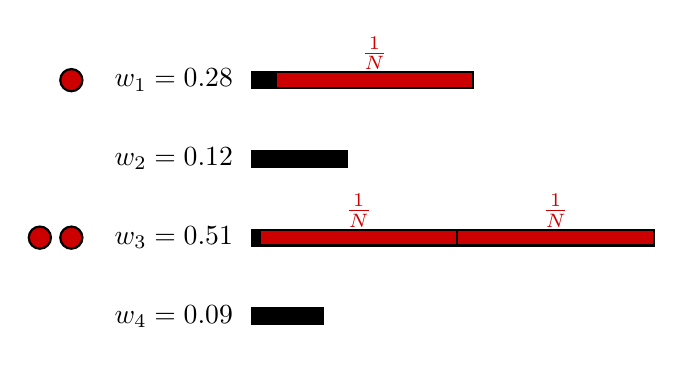
\begin{tikzpicture}
\node at (0,0) {$w_1=0.28$};
\node at (0,-1) {$w_2=0.12$};
\node at (0,-2) {$w_3=0.51$};
\node at (0,-3) {$w_4=0.09$};
\draw[thick, fill=black] (1,0.1) rectangle (1+0.28*10,-0.1);
\draw[thick, fill=black] (1,0.1-1) rectangle (1+0.12*10,-0.1-1);
\draw[thick, fill=black] (1,0.1-2) rectangle (1+0.51*10,-0.1-2);
\draw[thick, fill=black] (1,0.1-3) rectangle (1+0.09*10,-0.1-3);
\pause
\draw[thick,fill=darkred] (1+0.03*10,0.1) rectangle
node[above, color=darkred] {$\frac{1}{N}$} (1+0.28*10,-0.1);
\draw[thick, fill=darkred] (1+0.01*10,0.1-2) rectangle 
node[above, color=darkred] {$\frac{1}{N}$} (1+0.26*10,-0.1-2);
\draw[thick, fill=darkred] (1+0.26*10,0.1-2) rectangle 
node[above, color=darkred] {$\frac{1}{N}$} (1+0.51*10,-0.1-2);
\pause
\draw[thick, fill=darkred] (-1.3,0) circle (4pt);
\draw[thick, fill=darkred] (-1.3,-2) circle (4pt);
\draw[thick, fill=darkred] (-1.7,-2) circle (4pt);
\end{tikzpicture}
%\end{center}
\end{frame}


\begin{frame}{Residual Resampling}{Illustration}
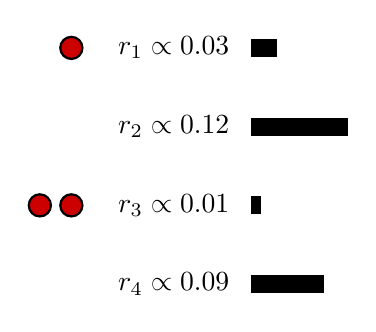
\begin{tikzpicture}
\draw[thick, fill=darkred] (-1.3,0) circle (4pt);
\draw[thick, fill=darkred] (-1.3,-2) circle (4pt);
\draw[thick, fill=darkred] (-1.7,-2) circle (4pt);
\node at (0,0) {$r_1 \propto 0.03$};
\node at (0,-1) {$r_2 \propto 0.12$};
\node at (0,-2) {$r_3 \propto 0.01$};
\node at (0,-3) {$r_4 \propto 0.09$};
\draw[thick, fill=black] (1,0.1) rectangle (1+0.03*10,-0.1);
\draw[thick, fill=black] (1,0.1-1) rectangle (1+0.12*10,-0.1-1);
\draw[thick, fill=black] (1,0.1-2) rectangle (1+0.01*10,-0.1-2);
\draw[thick, fill=black] (1,0.1-3) rectangle (1+0.09*10,-0.1-3);
\end{tikzpicture}
\end{frame}


\begin{frame}{Residual Resampling}{Illustration}
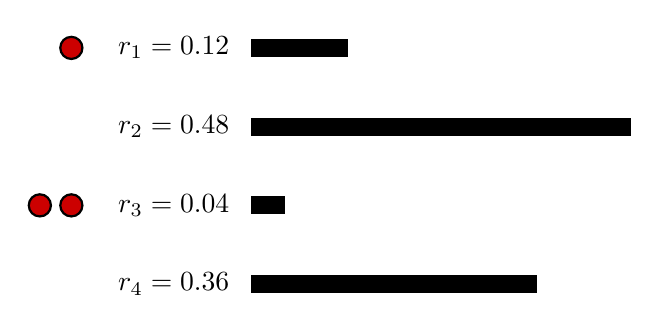
\begin{tikzpicture}
\draw[thick, fill=darkred] (-1.3,0) circle (4pt);
\draw[thick, fill=darkred] (-1.3,-2) circle (4pt);
\draw[thick, fill=darkred] (-1.7,-2) circle (4pt);
\node at (0,0) {$r_1 = 0.12$};
\node at (0,-1) {$r_2 = 0.48$};
\node at (0,-2) {$r_3 = 0.04$};
\node at (0,-3) {$r_4 = 0.36$};
\draw[thick, fill=black] (1,0.1) rectangle (1+0.03*40,-0.1);
\draw[thick, fill=black] (1,0.1-1) rectangle (1+0.12*40,-0.1-1);
\draw[thick, fill=black] (1,0.1-2) rectangle (1+0.01*40,-0.1-2);
\draw[thick, fill=black] (1,0.1-3) rectangle (1+0.09*40,-0.1-3);
\end{tikzpicture}
\end{frame}







\begin{frame}[allowframebreaks]{References}

{\small 
%\printbibliography
\bibliography{../../smc.bib}
}
\end{frame}
\end{document}